\chapter{Queryable Documents}\label{ch:queries}


\section{Developing a suitable representation}\label{sec:queries-representation}

\subsection{Requirements}\label{subsec:queries-requirements}

% TODO find a source on why we would want this specifically out of Confis
Assuming an existing document, being able to perform the following operations on said document is desirable: we will call these operations \emph{queries} (or questions) made to the contract.
In order to be accessible, these must be intuitive and should not require deep

% TODO justify this being common

\paragraph{Querying for Legal Capabilities} A common use-case is for a party to want to figure out their legal capabilities with respect to a contract, as well as the capabilities of other parties.
Take the example of a tenancy agreement: a tenant may want to know whether they are allowed to have pets, or whether the landlord is allowed to enter their property.

Therefore, a successful query system should be able to provide answers to questions such as \textit{`May $A$ do $X$?'}

A party may also have some requirements to be able to perform some action - such as performing a payment.
Continuing the example of the tenancy agreement, a landlord may be allowed to enter the premises in case of emergency, but not otherwise.
Thus, a more general question could be \emph{`Under what condition may $A$ do $X$?'}

\paragraph{Compliance verification} If figuring out a party's legal capabilities is a key part of dealing with a contract, so is figuring out their legal obligations.
Unlike a legal capability question, a compliance question cannot be formulated as \textit{`May $A$ do $X$?'} -- they should instead be along the lines of \textit{`What does X need to do in order to be compliant?'}.
We should also take into account that a party may have already done something to be compliant at the time of performing the query -- therefore we need to include some `state-of-the-world' in our question.
Additionally, parties usually interact and actions between more than a single party may be needed to achieve compliance.

Therefore, we can generalise a compliance verification question to \textit{`Given a series of past events S, what actions need to take place in order for the contract to be complied with?'}.

\subsection{Confis Internal Representation}\label{subsec:confis-ir}
As~\cite{knottenbeltContractDriven} notes, there is a clear compromise to be made between how complex a contract representation is, and how simple the computations needed to process it are.

Contrary to solutions discussed in~\autoref{sec:nlp} such as~\cite{sleimi2018NLP4}, Confis does not try to generalise a contract into a set of normative rules (as defined in~\autoref{eq:basic-rule}) straight away.
Instead, it tries to preserve all the information that goes into assembling a contract into an Intermediate Representation (that we will call \textbf{\emph{Confis IR}}).
The Confis IR is then converted into different sets of rules depending on the query being performed.

The Confis IR is a set of data structures, mostly tuples and collections, that can be mapped to a JSON or protobuf schema for serialisation.
For the sake of brevity, this report does not contain the entire schema, but see an example of a compiled IR at~\autoref{fig:confis:min-circumstance-ir}.


\section{Rule Generation and Contradiction Detection}\label{sec:rule-generation}

Given Confis evaluates different rules depending on the query from the IR, rather than generating rules from the DSL, generating rules from the IR is a critical part of Confis.

Confis has several types of clauses (see~\autoref{sec:language-semantics}) and each clause generates between one and four rules depending on the query type and its~\nameref{def:allowance}.
We will examine the example of converting a~\nameref{def:permission} clause with a non-empty~\nameref{def:circumstanceSet}.
It is a simple case that generates two rules.
Take the clause specified by~\autoref{fig:confis:aliceMayUseDataCClause} (the full contract can be found in~\autoref{fig:confis:min-circumstance}):


\begin{figure}[h]
    \centering
    \begin{minipage}{0.7\textwidth}
        \begin{minted}[
            autogobble,
            frame=lines,
            framesep=2mm,
        ]{kotlin}
    alice may use(data) asLongAs {
        within { (1 of June)..(30 of June) year 2022 }
    }
        \end{minted}
    \end{minipage}
    \caption{Clause with a Circumstance -- extract from~\autoref{fig:confis:min-circumstance}}
    \label{fig:confis:aliceMayUseDataCClause}
\end{figure}

The IR generated by this agreement can be found in~\autoref{fig:confis:min-circumstance-ir}.

We will now generate the rules for an \emph{allowance question} for this rule (ie, a query for legal capabilities).
As explained in the previous ~\autoref{subsec:queries-requirements}, the question can be formulated as \emph{`Given circumstances $C$, may Alice use the data?'}.
The inputs are a~\nameref{def:sentence} and a~\nameref{def:circumstanceSet}, while the output is a set Circumstance Sets (we require a Circumstance Set for each of the scenarios where Alice may use the data).
The resulting rules would
\begin{enumerate}
    \item Check whether it corresponds to a clause that matches the given question.
    \item Check whether the circumstances of the question are a specific case of those of the clause (in order to report a positive result).
    \item Check whether the question is not specific enough to be covered by the clause but concerns the same circumstances (in order to report an ambiguous result).
\end{enumerate}

Those rules are given by the pseudocode in~\autoref{fig:confis:aliceMayUseDataRule}:

\begin{figure}[h]
    \centering
    \begin{minted}[
        autogobble,
        frame=lines,
        framesep=2mm,
        fontsize=\small,
    ]{kotlin}
            AllowanceRule(
                // predicate: (Permission, Question, Result) -> Boolean
                when = { p, q, _ ->
                    p.sentence == q.sentence &&
                        p.circumstanceSet generalises q.circumstanceSet
                }
                // side-effect: (Permission, Result) -> Void
                then = { p, r -> result = Allow }
            ),
            // question general enough to concern us but not narrow enough to match clause
            AllowanceRule(
                when = { p, q, _ ->
                    p.sentence == q.sentence &&
                        !(p.circumstanceSet generalises q.circumstanceSet)  &&
                        p.circumstances overlapsWith q.circumstances
                },
                then = { if (result != Allow) result = Depends },
            )
    \end{minted}
    \caption{Rules generated from the clause given in~\autoref{fig:confis:aliceMayUseDataCClause}}
    \label{fig:confis:aliceMayUseDataRule}
\end{figure}

Rules can be combined this way in order to construct the Result.
Because the rules engine Confis uses allows continuous rule evaluation~(see~\autoref{subsec:j-easy-rules}) we can add more rules that compare the rules generated by different clauses in order to detect contradictions in the clauses.
% TODO screenshot of contradiction detection!!
This allows detecting malformed contracts by detecting contradictions that, while they are semantically and syntactically correct, make little sense.

An example for such an agreement can be found in~\autoref{fig:confis:contradictions-example}.
We are able to detect such a contradiction thanks to the \texttt{overlapsWith} function for Circumstance Sets, which is discussed in~\autoref{subsec:circumstance}.


\begin{figure}[h]
    \centering
    \begin{minted}[
        autogobble,
        frame=lines,
        framesep=2mm,
    ]{kotlin}
    alice mayNot use(data) asLongAs {
        val year2022 = (1 of January)..(31 of December) year 2022
        within { year2022 }
    }
    alice may use(data) asLongAs {
        within { (1 of June)..(30 of June) year 2022 }
    }
    \end{minted}
    \caption{A correct Confis agreement that contains detectable contradictions}
    \label{fig:confis:contradictions-example}
\end{figure}


% TODO examples of DSL -> IR and IR -> rules


\section[Query UI]{Tooling for Accessible Querying: the Query UI}\label{sec:queryUI}

A core distinctive capability of Confis is its~\nameref{def:accessibility} -- a contract drafter should not need to use a command-line tool or an HTTP API in order to perform a query.
In order to meet this requirement, the Confis Plugin~(which is an extension to the IntelliJ IDE~\cite{intelliJRepo, ideaExtensionPoints}) provides a graphical user interface to construct and display questions.

The user experience is as follows: the contract drafter writes their agreement into the Confis Editor~(see~\autoref{sec:confis-editor}) and, on the side, they have a window that allows performing queries on the contract they are writing.
This allows them to perform queries and check whether their answers are within the drafter's expectations.

\subsection{Query UI Implementaiton}\label{subsec:query-ui-implementaiton}

Implementing a UI to build queries involves:

\begin{itemize}
    \item Constructing a Sentence through a UI
    \item Constructing a Circumstance Set through a UI
    \item (therefore) Constructing a Circumstance through a UI
    \item Compiling and generating rules from the agreement in the Confis Editor
    \item Displaying the result from the rules' evaluation in an English-readable fashion
\end{itemize}

Out of all of these, constructing a Circumstance proved to be an interesting challenge.
This section will go into more detail about how this was done as an example of overcoming some of the technical difficulty in developing the prototype.

At the time of writing Confis has four different types of Circumstance, and is designed to be able to accommodate any number.
It would not have been desirable to require designing a UI for each new Circumstance.

According to~\cite{fowlerLangWorkbench} designing a user interface to assemble queries with the concepts described in~\autoref{sec:language-semantics} is much like building a new DSL, except it is a visual one instead of a textual one.
The solution to the difficulty of making a UI for assembling Circumstances proved to be in combining the textual DSL that is a Confis agreement, and the visual one that is the query UI\@.
The end result allows building questions through a UI without having to require a command-line interface or calling a library from code, and permits writing Circumstances as code just like they would be written in an agreement.

Allowing the user to type in Circumstances in a text box involves creating a synthetic Abstract Syntax Tree (AST) of the Kotlin language (which Confis is based on, see~\autoref{subsec:dsl-implementation} for more details) which includes the necessary imports for the DSL, and then compiling this language fragment in order to instantiate a Circumstance Set in memory.
This synthetic Circumstance Set can then be passed to the query engine for rule generation.

While the goal of assembling a Circumstance has been achieved, the Circumstance editor in the query UI is far from being on-par with the main Confis Editor (discussed in~\autoref{sec:confis-editor}, it provides compiler error reporting, autocompletion, and syntax highlighting).
We decided to make intelligent editing inside the Circumstance editor a priority, because the only other way to inform the user about malformed circumstance code would be to expose them to the Kotlin Compiler logs.
In order to achieve this, Confis reuses the open-source implementation of IntelliJ's Java expression evaluator~\cite{intelliJRepo}~(meant to be used inside debugging sessions).
It parses the Circumstance editor and constructs a new AST which is then instantiated in a new program.
The program is then fed to the debugging evaluator, which is then able to provide relevant editing hints to the user.
Upon changes of the Confis script or the Circumstance test box content, the synthetic AST is reconstructed so the editor can provide up-to-date aid.

This end result is a smart Circumstance editor on par with the normal contract editor, able to report compilation errors and aware of the symbols present in the contract.
This is shown in~\autoref{fig:queryUi-geophys-window}.


\tikzset{font={\fontsize{8pt}{9}\selectfont}}
\begin{figure}[h]
    \usetikzlibrary{shapes.misc, arrows.meta}
    \colorlet{pastelBlue}{blue!40!white}
    \begin{tikzpicture}
    [
        node distance=1.6cm and 1.4cm,
    ]

        \node (textBox) [
            draw,
            align=left,
            rectangle,
            rounded corners,
            rectangle,
            text width=3.6cm,
        ] {
            \textbf{Circumstance editor text box}\\
            Contains circumstance code:
            \vspace{-6mm}
            \begin{minted}[autogobble]{kotlin}
                after {
                    alice did pay(bob)
                }
            \end{minted}
        };
        \node (queryUi) [
            draw,
            align=left,
            rectangle,
            rounded corners,
            rectangle,
            left=of textBox,
        ] {
            \textbf{Query UI}\\
            Contains\\dropdowns\\
            to assemble\\question
        };

        \node (editor) [
            draw,
            align=left,
            rectangle,
            rounded corners,
            rectangle,
            right=of textBox,
            text width=4cm,
        ] {
            \textbf{Confis Contract Editor}\\
            Contains file contents of Confis contract:
            \vspace{-2mm}
            \begin{minted}[autogobble]{kotlin}
                val alice by party
                val bob by party
                val pay by action
                // ...
            \end{minted}
        };

        \node (compiler1) [
            draw,
            align=left,
            rectangle,
            rounded corners,
            rectangle,
            below=of textBox,
        ] {
            \textbf{Circumstance Compiler}\\
            see:\\~\autoref{subsec:dsl-implementation}
        };


        \node (synth1) [
            align=left,
            rectangle,
            below=of editor,
        ] {Synthetic AST};

        \node (compiler2) [
            draw,
            align=left,
            rectangle,
            rounded corners,
            rectangle,
            right=of synth1,
        ] {
            \textbf{Contract Compiler}\\
            see:\\~\autoref{subsec:dsl-implementation}
        };

        \node (eval) [
            draw,
            align=left,
            rectangle,
            rounded corners,
            rectangle,
            below=of synth1,
        ] {
            \textbf{Java Debugging Expression Evaluator}\\
            Provides editing context to an AST
        };
        \node (synth2) [
            align=center,
            rectangle,
            left=of compiler1,
        ] {Assembled\\Question};

        \node (queryEngine) [
            draw,
            align=left,
            rectangle,
            rounded corners,
            rectangle,
            below=of synth2,
        ] {
            \textbf{Query Engine}\\
            see~\autoref{sec:rule-generation}
        };


        \draw[->]
        (textBox.270+50)
        to [out=270+30,in=90+30]
        node [align=center, fill=white]{Circumstance\\code}
        (synth1.90+70);

        \draw[->]
        (eval.90+30)
        to [out=90+30,in=-90+30]
        node [align=center, fill=white]{Editor\\Hints}
        (textBox.-60);

        \draw[->] (textBox.south)
        -- node[align=center, fill=white] { Synthetic\\AST }
        (compiler1);

        \draw[->] (compiler1.90+55)
        to [out=90+45,in=90-45]
        node[align=center, fill=white, yshift=0.2cm] { Instantiated\\circumstance }
        (synth2.90-45);

        \draw[->] (editor.south)
        -- node[align=center, fill=white] { Contract code }
        (synth1);

        \draw[->] (synth1.south)
        -- node {}
        (eval);

        \draw[->] (synth2.south)
        -- node {}
        (queryEngine);

        \draw[->] (queryUi.south)
        -- node[align=center, fill=white] {Question\\selection}
        (synth2);

        \draw[->]
        (editor.east)
        to [out=0,in=90]
        node [align=center, fill=white]{Contract\\code}
        (compiler2);

        \draw[->]
        (compiler2.south)
        to [out=270,in=0]
        node [align=center, fill=white]{IR}
        (queryEngine);

        \draw[->]
        (queryEngine.90+30)
        to [out=90+65,in=-90-20]
        node [align=center, fill=white, xshift=4mm, yshift=-12mm]{Result}
        (queryUi);


    \end{tikzpicture}
    \caption
    [Diagram of the Query UI's Circumstance editor]
    {Diagram showing the architecture behind the Query UI's Circumstance editor}
    \label{fig:circumstance-editor-arch}
\end{figure}

\begin{figure}[h]
    \centering
    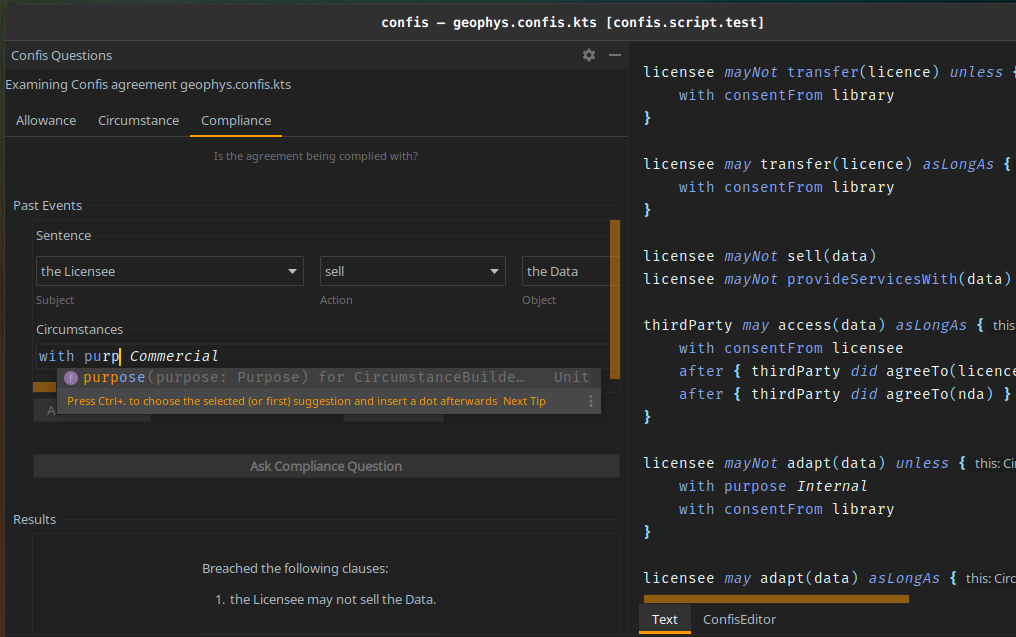
\includegraphics[width=\textwidth]{figures/geophys.confis.queryUI}
    \caption[Query UI window for Geophysical Libray License]{
        Query UI window for agreement given in~\autoref{fig:confis:geophys}

        \par\small
        Note how the question is built by selecting the \emph{Compliance} tab and assembling the Sentence \emph{`the Licensee sell the Data'} from dropdown menus.
        Circumstances are built through the text box, featuring autocompletion and compliance checking
    }
    \label{fig:queryUi-geophys-window}
\end{figure}

More screenshots can be found in the appendix under~\autoref{sec:app:confis-query-ui}, demonstrating an Allowance question and a compile error in the Circumstances editor text box.


\section{Confis as a Generalisation of Ricardian Contracts}\label{sec:generalisation-of-ricardian-contracts}

Ricardian Contracts~\cite{grigg2004ricardian} (discussed in~\autoref{subsec:ricardian-contracts}) are one of the few technologies in the state of the art discussed in the~\nameref{ch:background} chapter and allow querying a contract and are concerned with the~\nameref{def:accessibility} requirement at all.

Confis tries to capture the meaning of the agreement it encodes.
For example, a party should be able to query about their compliance with the contract without needing to know whether the contract is a tenancy agreement, a bond, or a license.
A Ricardian contract, on the other hand, is closer to an instance of a specific kind of contract -- therefore knowledge about the contract `type', or `template', are necessary to extract the metadata encoded in it.

This project is a generalisation of Ricardian contracts in that Confis agreements meet all the requirements given by definition of~\nameref{def:ricardian}\footnote{It is worth noting that while Confis as a formalism does meet the requirements given by the definition of a~\nameref{def:ricardian}, the artefacts included in the project do not implement the public-key signing infrastructure (discussed in~\autoref{subsec:crypto:pubkey}).}, but it also tries to convey and capture the meaning of the contract, so that both a machine and a human can take every single possible state into account.

Another crucial difference from what was first specified by Grigg in~\cite{grigg2004ricardian} is that Confis does not intend to let a user write legal prose.
Rather, it hopes to produce machine-generated but human-readable prose legal prose from its internal encoding of the agreement -- see~\autoref{sec:additional-tooling:doc-rendering} for a discussion of this feature.
